% enju — workflow-run hero figure for the README.
%
% A representative (hypothetical, domain-neutral) run: one root task
% fans out with for_each, each item is processed and checked, results
% fan back in (collects), a human gates the deliverable, and publish
% lays it onto the base branch. Executors are colour-coded
% (human / agent / script) and every accepted task is a git commit.
%
% Style palette is shared with the preprint (preprint/main.tex) so the
% README and the paper read as one system.
%
% Render:  make            (-> workflow.svg + workflow.png)
% or:      pdflatex workflow.tex && pdf2svg workflow.pdf workflow.svg
\documentclass[border=10pt]{standalone}
\usepackage{lmodern}
\usepackage{tikz}
\usetikzlibrary{shapes,arrows,positioning,fit,backgrounds,calc}

\begin{document}
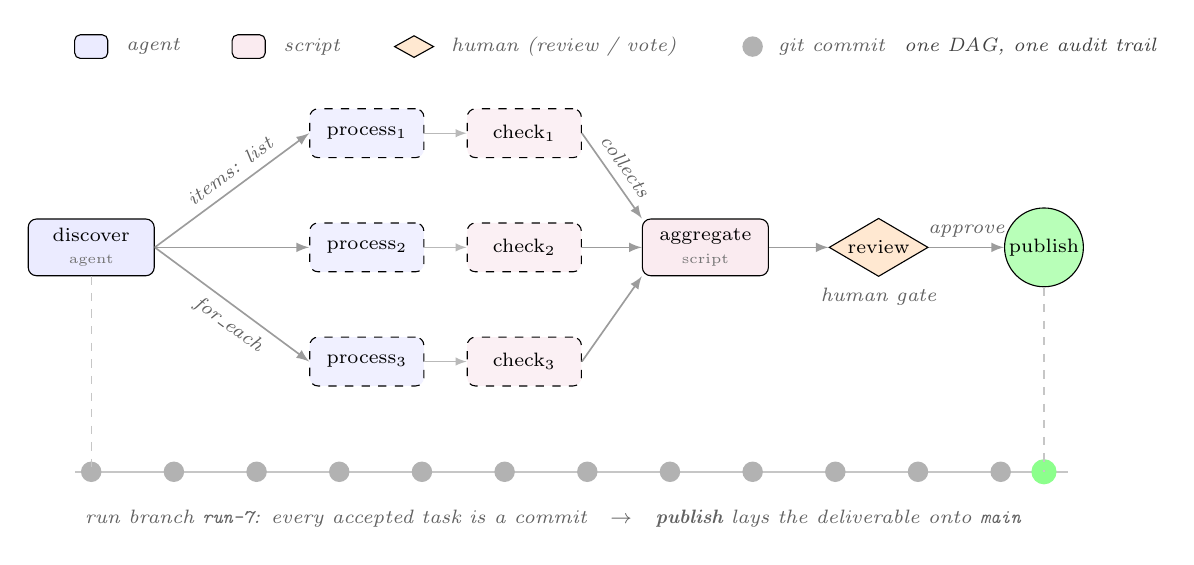
\begin{tikzpicture}[
    font=\small,
    agent/.style={rectangle, rounded corners=3pt, draw, fill=blue!8,
        minimum width=1.6cm, minimum height=0.72cm, font=\scriptsize, align=center, inner sep=2pt},
    script/.style={rectangle, rounded corners=3pt, draw, fill=purple!8,
        minimum width=1.6cm, minimum height=0.72cm, font=\scriptsize, align=center, inner sep=2pt},
    iter/.style={rectangle, rounded corners=3pt, draw, dashed, fill=blue!6,
        minimum width=1.45cm, minimum height=0.62cm, font=\scriptsize, align=center, inner sep=2pt},
    iterc/.style={rectangle, rounded corners=3pt, draw, dashed, fill=purple!6,
        minimum width=1.45cm, minimum height=0.62cm, font=\scriptsize, align=center, inner sep=2pt},
    gate/.style={diamond, draw, fill=orange!18, aspect=1.7,
        font=\scriptsize, align=center, inner sep=1pt},
    term/.style={circle, draw, fill=green!28, minimum size=1.0cm,
        font=\scriptsize, align=center, inner sep=1pt},
    commit/.style={circle, fill=gray!60, minimum size=2.6mm, inner sep=0pt, draw=none},
    flow/.style={->, >=latex, gray!78, semithick},
    feflow/.style={->, >=latex, gray!55, thin},
    lbl/.style={font=\scriptsize\itshape, text=black!62},
    sw/.style={rectangle, rounded corners=2pt, draw, minimum width=0.42cm, minimum height=0.3cm, inner sep=0pt},
]

% ---------- root ----------
\node[agent] (disc) at (0,0) {discover\\\textcolor{black!55}{\tiny agent}};

% ---------- for_each fan-out ----------
\node[iter]  (d1) at (3.5, 1.45) {process$_1$};
\node[iter]  (d2) at (3.5, 0.0)  {process$_2$};
\node[iter]  (d3) at (3.5,-1.45) {process$_3$};

\node[iterc] (c1) at (5.5, 1.45) {check$_1$};
\node[iterc] (c2) at (5.5, 0.0)  {check$_2$};
\node[iterc] (c3) at (5.5,-1.45) {check$_3$};

\draw[flow] (disc.east) -- node[lbl, above, pos=0.55, sloped] {items: list} (d1.west);
\draw[flow] (disc.east) -- (d2.west);
\draw[flow] (disc.east) -- node[lbl, below, pos=0.55, sloped] {for\_each} (d3.west);
\draw[feflow] (d1) -- (c1);
\draw[feflow] (d2) -- (c2);
\draw[feflow] (d3) -- (c3);

% ---------- collects (fan-in) ----------
\node[script] (agg) at (7.8,0) {aggregate\\\textcolor{black!55}{\tiny script}};
\draw[flow] (c1.east) -- node[lbl, above, pos=0.5, sloped] {collects} (agg.north west);
\draw[flow] (c2.east) -- (agg.west);
\draw[flow] (c3.east) -- (agg.south west);

% ---------- human gate ----------
\node[gate] (rev) at (10.0,0) {review};
\draw[flow] (agg.east) -- (rev.west);
\node[lbl, below=0.5pt of rev] {human gate};

% ---------- publish ----------
\node[term] (pub) at (12.1,0) {publish};
\draw[flow] (rev.east) -- node[lbl, above, pos=0.5] {approve} (pub.west);

% ---------- git ribbon ----------
\def\ribY{-2.85}
\draw[gray!45, semithick] (-0.2,\ribY) -- (12.4,\ribY);
\foreach \x in {0,1.05,...,12.0} { \node[commit] at (\x,\ribY) {}; }
\node[commit, fill=green!45, minimum size=3.2mm] at (12.1,\ribY) {};
\node[lbl, anchor=west, align=left] at (-0.2,-3.45)
  {run branch \texttt{run-7}: every accepted task is a commit\quad$\rightarrow$\quad
   \textbf{publish} lays the deliverable onto \texttt{main}};
\draw[gray!45, dashed] (disc.south) -- (0,\ribY);
\draw[gray!45, dashed] (pub.south) -- (12.1,\ribY);

% ---------- executor legend ----------
\begin{scope}[shift={(0,2.55)}]
  \node[sw, fill=blue!8]   (lA) at (0,0) {};   \node[lbl, anchor=west] at (0.32,0) {agent};
  \node[sw, fill=purple!8] (lS) at (2.0,0) {}; \node[lbl, anchor=west] at (2.32,0) {script};
  \node[diamond, draw, fill=orange!18, aspect=1.7, minimum width=0.5cm, minimum height=0.28cm, inner sep=0pt] (lH) at (4.1,0) {};
  \node[lbl, anchor=west] at (4.45,0) {human (review / vote)};
  \node[commit] (lC) at (8.4,0) {}; \node[lbl, anchor=west] at (8.6,0) {git commit};
  \node[lbl, anchor=west, text=black!75] at (10.2,0) {one DAG, one audit trail};
\end{scope}

\end{tikzpicture}
\end{document}
